\documentclass[
  luatex,
  report,
  a4paper,
  11pt,
  jlreq_notes,
]{jlreq}

% jlreqsetupで色々設定できるようにする
\usepackage{jlreq-complements}

% jlreqの設定
\jlreqsetup{
  thebibliography_heading={  % 参考文献の見出しの出力命令を設定
    \chapter*{\refname}    % 見出しを章にする
    \addcontentsline{toc}{chapter}{\refname}    % 目次に追加
  },
}

% =============================================================================
% 基本パッケージ
% =============================================================================
\usepackage{xcolor}
\usepackage{graphicx}

% =============================================================================
% 数式
% =============================================================================
\usepackage{amsmath,amssymb}
\usepackage{mathtools}
% \mathtoolsset{showonlyrefs=true} % 参照した数式番号のみを表示する
\usepackage{siunitx}  % 単位付き数値の入力を楽にする
\usepackage[version=4]{mhchem}
\usepackage{physics2} % 数式の記述を楽にする
\usephysicsmodule{ab}   % 括弧のサイズを自動調整する
% 行列の記述を楽にする
\usephysicsmodule{diagmat}
\usephysicsmodule{xmat}
\usepackage{derivative}   % 微分記号の入力を楽にする

\usepackage[
  % mathtoolsと一部競合するため，警告を無視
  warnings-off={mathtools-colon,mathtools-overbracket}
]{unicode-math}
\unimathsetup{math-style=TeX,bold-style=TeX}
\setmainfont[Ligatures=TeX]{Latin Modern Roman}
\setsansfont[Ligatures=TeX]{Latin Modern Sans}
\setmonofont{Latin Modern Mono}
\setmathfont{Latin Modern Math}

\usepackage[
  noto-serif-jp,  % ヒラギノ明朝(プロポーショナル)を使用
  deluxe,  % 多ウェイト化を有効にする
  % jlreqで使えるようにする
  jfm_yoko=jlreq,
  jfm_tate=jlreqv,
]{luatexja-preset}
% \ltjsetparameter{jacharrange=full}
% \setsansfont{Latin Modern Sans}
% \setsansjfont{IPAexGothic}
% \setmonofont{Latin Modern Mono}
% 和文（jsarticle 既定相当）
% \setmainjfont[
%     UprightFont   = {Noto Sans JP Regular},   % 通常
%     BoldFont      = {Noto Sans JP Bold},      % 太字
%     MediumFont    = {Noto Sans JP Medium},    % 中太
%     SemiBoldFont  = {Noto Sans JP SemiBold},  % セミボールド
%     BlackFont     = {Noto Sans JP Black},     % 黒字
%     LightFont     = {Noto Sans JP Light},     % 細字
%     ExtraLightFont= {Noto Sans JP ExtraLight},% 極細
%     ExtraBoldFont = {Noto Sans JP ExtraBold}  % 超太字
% ]{Noto Sans JP Regular}

\usepackage{booktabs} % 表の罫線を扱う
\usepackage{multirow}
\usepackage{multicol}
\usepackage{enumitem}
\usepackage{float}

% キャプションを設定
\usepackage[hang,small,bf]{caption}
\usepackage[subrefformat=parens]{subcaption}
% \captionsetup[subfigure]{labelformat=simple}
\renewcommand{\thesubfigure}{\alph{subfigure}}

% ソースコードを扱う
\usepackage{listings}
\lstset{
  tabsize={4}, % タブの展開後のサイズ
  numbers=left, % 行番号表示，デフォルト: none 他のオプション: left, right
  basicstyle={\small},   % 識別子の書体指定
  identifierstyle={\small},  % 識別子の書体指定
  %numberstyle=\scriptsize,  % 行番号の書体指定
  commentstyle={\small\ttfamily},  % 注釈の書体。
  ndkeywordstyle={\small},
  keywordstyle={\small\bfseries},  % キーワードの書体指定。
  stringstyle={\small\ttfamily},
  columns=[l]{fullflexible},
  xrightmargin=0\zw,
  xleftmargin=0\zw,
  numbersep=1\zw,
  %backgroundcolor={\color[gray]{.85}},
  frame=lines,  % frameの指定．デフォルト: none 他のオプション: leftline, topline, bottomline, lines, single, shadowbox
  breaklines=true,  % 行が長くなってしまった場合の改行．デフォルト: false
}
\floatplacement{figure}{!htbp}
\floatplacement{table}{!htbp}


% =============================================================================
% 参考文献（natbib + BibTeX）
% =============================================================================
\usepackage[
  backend=biber,
  style=numeric,
  sorting=none]{biblatex}

% \DefineBibliographyStrings{japanese}{
%   andothers={他} % 和文文献の "et al." 相当
% }
% \DefineBibliographyStrings{english}{
%   andothers={\textit{et al.}} % 欧文文献
% }

% ラベル形式
\DeclareFieldFormat{labelnumberwidth}{[#1]\hspace{0.5em}}

% 左マージンなどの調整
\setlength{\biblabelsep}{0pt}
\setlength{\bibitemsep}{0pt}
\setlength{\bibparsep}{0pt}

% フォーマットを文献タイプ別に分ける
\DeclareFieldFormat[article]{title}{%
  \iffieldequalstr{langid}{japanese}{「#1」}{\textit{#1}}%
}
\DeclareFieldFormat[book]{title}{%
  \iffieldequalstr{langid}{japanese}{『#1』}{\textit{#1}}%
}
\DeclareFieldFormat{journaltitle}{%
  \iffieldequalstr{langid}{japanese}{#1}{\textit{#1}}%
}
\DeclareFieldFormat{booktitle}{%
  \iffieldequalstr{langid}{japanese}{#1}{\textit{#1}}%
}

% "In:" マクロを削除
\renewbibmacro{in:}{}

% 欧文・和文で連名の区切りを制御
\DeclareDelimFormat{finalnamedelim}{%
  \ifnumgreater{\value{liststop}}{2}{\finalandcomma}{}%
  \addspace\multinamedelim
}

% Bib ファイルの登録
\addbibresource{reference.bib}

% =============================================================================
% その他
% =============================================================================
\usepackage{comment}
\usepackage{url}
\usepackage{indentfirst}

% =============================================================================
% ハイパーリンク
% =============================================================================
\usepackage[hidelinks]{hyperref}
\usepackage{cleveref}

\crefname{figure}{図}{図}
\Crefname{figure}{図}{図}

\crefname{table}{表}{表}
\Crefname{table}{表}{表}

\crefname{equation}{式}{式}
\Crefname{equation}{式}{式}

\crefname{inlineitem}{}{}
\Crefname{inlineitem}{}{}

\crefformat{equation}{(#2#1#3)式}
\Crefformat{equation}{(#2#1#3)式}
\crefrangeformat{equation}{(#3#1#4)–(#5#2#6)式}
\crefmultiformat{equation}
  {(#2#1#3)式}
  {, (#2#1#3)式}
  {, (#2#1#3)式}
  {, (#2#1#3)式}
\crefrangemultiformat{equation}
  {(#3#1#4)–(#5#2#6)式}
  {, (#3#1#4)–(#5#2#6)式}
  {, (#3#1#4)–(#5#2#6)式}
  {, (#3#1#4)–(#5#2#6)式}
\crefformat{inlineitem}{%
  \textcircled{\scriptsize#2#1#3}%
}

% 図表周りの空間調整
\renewcommand{\textfloatsep}{10pt}  % 図表と本文の間隔（ページ上端・下端）
\renewcommand{\floatsep}{10pt}      % 図表同士の間隔
\renewcommand{\intextsep}{5pt}     % 本文中に置かれた図表との間隔
\renewcommand{\belowcaptionskip}{5pt}
  
% =============================================================================
% 諸設定
% =============================================================================
% 和文用タイトル再設定
\renewcommand{\figurename}{図}
\renewcommand{\tablename}{表}
\renewcommand{\contentsname}{目次}
\renewcommand{\listfigurename}{図目次}
\renewcommand{\listtablename}{表目次}
\renewcommand{\baselinestretch}{0.95}  % 行間調整

% =============================================================================
%　マクロ
% =============================================================================
% Keep same float settings as original
\newcounter{inlineitem}
\newcommand{\inlineitem}[1]{%
	\refstepcounter{inlineitem}%
	\label{#1}%
	\space\textcircled{\scriptsize\theinlineitem}%
}
\newcommand{\dd}{\mathop{}\!\mathrm{d}}
\newcommand{\subrm}[2]{\ensuremath{#1_{\mathrm{#2}}}}
\newcommand{\cntmerr}{\ensuremath{\varepsilon_{\mathrm{cntm}}}}
\newcommand{\staterr}{\ensuremath{\varepsilon_{\mathrm{stat}}}}

% % 日本語用マクロ（目次やPDF文字列も安全）
% \newcommand{\n2sO2sJ}{\texorpdfstring{\ce{N2}ストークス散乱波長と\ce{O2}ストークス散乱波長}{N2 Stokes, O2 Stokes}}
% \newcommand{\n2sO2aJ}{\texorpdfstring{\ce{N2}ストークス散乱波長と\ce{O2}アンチストークス散乱波長}{N2 Stokes, O2 a-Stokes}}
% \newcommand{\n2sN2aJ}{\texorpdfstring{\ce{N2}ストークス散乱波長と\ce{N2}アンチストークス散乱波長}{N2 Stokes, N2 a-Stokes}}
% \newcommand{\n2aO2aJ}{\texorpdfstring{\ce{N2}アンチストークス散乱波長と\ce{O2}アンチストークス散乱波長}{N2 a-Stokes, O2 a-Stokes}}
% \newcommand{\o2sN2aJ}{\texorpdfstring{\ce{O2}ストークス散乱波長と\ce{N2}アンチストークス散乱波長}{O2 Stokes, N2 a-Stokes}}
% \newcommand{\o2sO2aJ}{\texorpdfstring{\ce{O2}ストークス散乱波長と\ce{O2}アンチストークス散乱波長}{O2 Stokes, O2 a-Stokes}}

% % 英語用マクロ
% \newcommand{\n2sO2sE}{\ce{N2} Stokes, \ce{O2} Stokes}
% \newcommand{\n2sO2aE}{\ce{N2} Stokes, \ce{O2} a-Stokes}
% \newcommand{\n2sN2aE}{\ce{N2} Stokes, \ce{N2} a-Stokes}
% \newcommand{\n2aO2aE}{\ce{N2} a-Stokes, \ce{O2} a-Stokes}
% \newcommand{\o2sN2aE}{\ce{O2} Stokes, \ce{N2} a-Stokes}
% \newcommand{\o2sO2aE}{\ce{O2} Stokes, \ce{O2} a-Stokes}

% =============================================================================

\begin{document}
\begin{titlepage}
\begin{center}
    \Large{令和7年度 修士論文}

    \vspace{7\zw}

    \huge{\textgt{
        火山ガス中二酸化硫黄分布観測のための\\
        ラマンDIALの検討
    }}

    \vspace{1\zw}

    \Large{\bfseries
        Simulation study on Raman DIAL system\\
        for volcanic sulfur dioxide measurement
    }

    \vspace{3\zw}

    \Large{
        東京都立大学\\
        システムデザイン研究科\\
        電子情報システム工学域
    }

    \vspace{3\zw}

    \Large{24861657 平山拓道}

    \vspace{1\zw}

    \Large{指導教員 柴田泰邦 教授}
\end{center}
\end{titlepage}

\pagenumbering{roman}
\tableofcontents

\clearpage
\listoffigures
\listoftables

\clearpage
\pagenumbering{arabic}
\chapter[研究背景]{序論}\label{chapt1}
本章では, 火山ガスの危険性およびその監視手法について概説し, 既存手法の課題を踏まえた上で, 本研究で提案するラマンDIALの位置付けと研究目的を述べる.
\section{火山ガスの監視方法}
日本列島は, 複数のプレート（太平洋,フィリピン海,北米,ユーラシア）が
相互に沈み込み,
衝突する世界的にも稀な地質構造を有している. 
このようなプレート境界が集中する地理的条件により,
日本は地殻変動や火山活動が極めて活発な地域となっている. 
その結果, 日本は世界有数の火山大国として知られている. 
\cref{fig:volcano_dist}に示す世界の活火山の分布状況を見ると,
世界全体に存在する約1500の活火山のうち,
約7\%に相当する111山が日本国内に集中しており,
日本列島が火山活動の影響を強く受ける地域であることが分かる\cite{bousai2021}. 
このような背景から, 日本では火山災害にたびたび見舞われてきた.
\begin{figure}
    \centering
    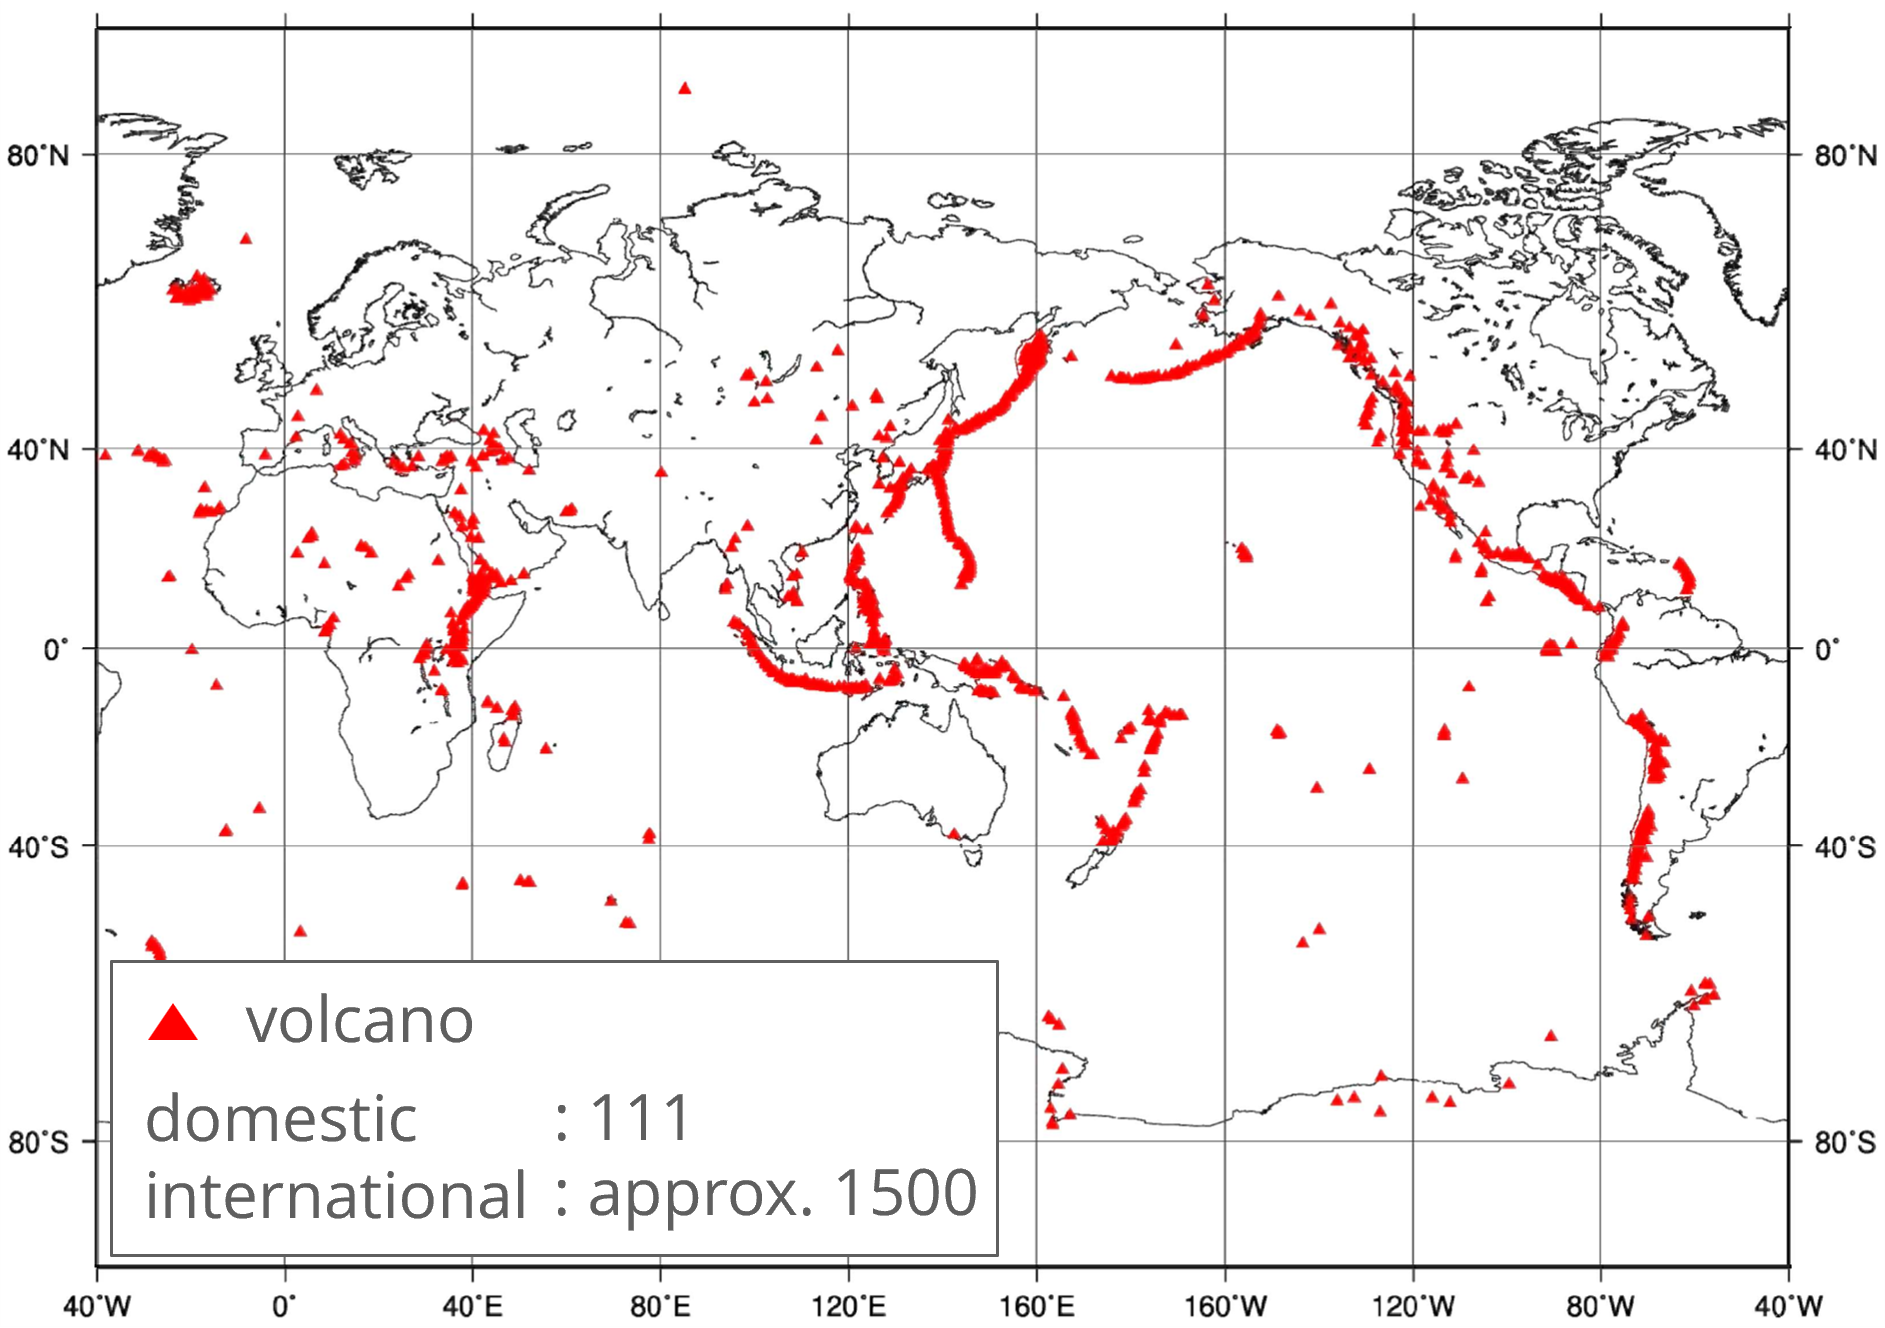
\includegraphics[width=0.6\linewidth]{fig/volcano_distribution.png}
    \caption{世界の活火山分布}
    \label{fig:volcano_dist}
\end{figure}

\newpage
火山災害には噴石や火砕流, 降灰など様々な形態が存在するが, 
火山ガスもまた重大な災害要因の一つである。過去100年間において,
火山ガスに起因する死亡者数は約1900人にのぼると報告されており,
火山ガスの危険性は決して小さくない\cite{Hirabayashi2003VolcanicGas}. 
火山ガスの中でも,二酸化硫黄（\ce{SO2}）は特に強い毒性を有する気体である. 
\cref{tab:SO2_toxicity}に\ce{SO2}の人体への影響を示す.
\begin{table}
    \centering
    \caption{二酸化硫黄の危険性}
    \label{tab:SO2_toxicity}
    \begin{tabular}{c|c}
        濃度[\unit{ppm}] & 人体への影響 \\
        \hline
        5 & 刺激症状（咳, 喉の痛み） \\
        30\sim40 & 呼吸困難 \\
        400\sim500 & 嗅覚が侵され, 臭気を知覚できない \\
        500 ppm\sim & 致死濃度\\
    \end{tabular}
\end{table}

\noindent
\ce{SO2}は,濃度が5 ppmを超えると呼吸器系への刺激が確認され,
30～40 ppmでは呼吸が困難となる. 
さらに,400 ppmを超える高濃度環境では生命に危険が及ぶことが知られている. 
その上, 強い毒性によって嗅覚が麻痺し, 特徴的な臭気を感知できなくなるため,
被害が拡大しやすいという性質も持ち合わせている.
実際, 環境基準としては, 環境基本法に基づき, 
% 「人の健康を保護し、生活環境を保全するうえで維持されることが望ましい基準」として
1時間値の1日平均値が\qty{0.04}{ppm}以下であり,
かつ, 1時間値が\qty{0.1}{ppm}以下であることと定められており, 
許容濃度としては, ACGIH\footnote{
    米国産業衛生専門家会議:American Conference of Governmental Industrial Hygienists
}が
通常の労働\footnote{
    1日8時間, 週40時間程度で肉体的に激しくない労働を指す. 
}
で, 平均暴露濃度が\qty{2}{ppm}以下であれば
ほとんどの労働者に健康上の悪い影響が見られないと判断している\cite{miyake}. 
平均暴露濃度は呼吸保護具を装着していない状態で
吸入するであろう濃度のことである. 
大気中の二酸化炭素濃度が約\qty{425}{ppm}前後であることを考えると,
\ce{SO2}が極めて低濃度で人体に深刻な影響を及ぼす強毒性ガスであることが分かる. 
加えて,\ce{SO2}は大気中で反応し,エアロゾルや硫酸ミストを形成する場合があり,
これらによる視程障害や呼吸器系への影響などの二次的被害も無視できない\cite{miyake}. 
そのため,三宅火山や霧島火山などでは,
火山性ガスの継続的な監視が実施されている。

\newpage
火山ガス観測には,電気化学式センサが広く用いられている. 
電気化学式センサは,測定対象ガスと触媒との電気化学反応量から気体濃度を推定する
微量気体濃度計であり,噴気が放出される地点に設置して測定が行われる. 
本手法は定点観測を前提としているため, 
気体濃度の空間分布を把握することができないという課題がある. 
また,反応が定常状態に達するまで濃度を評価できないことから,
時間的に連続した測定が困難であり,
人的被害を防ぐために継続して監視するにはこの課題も重要である.

\begin{figure}
    \centering
    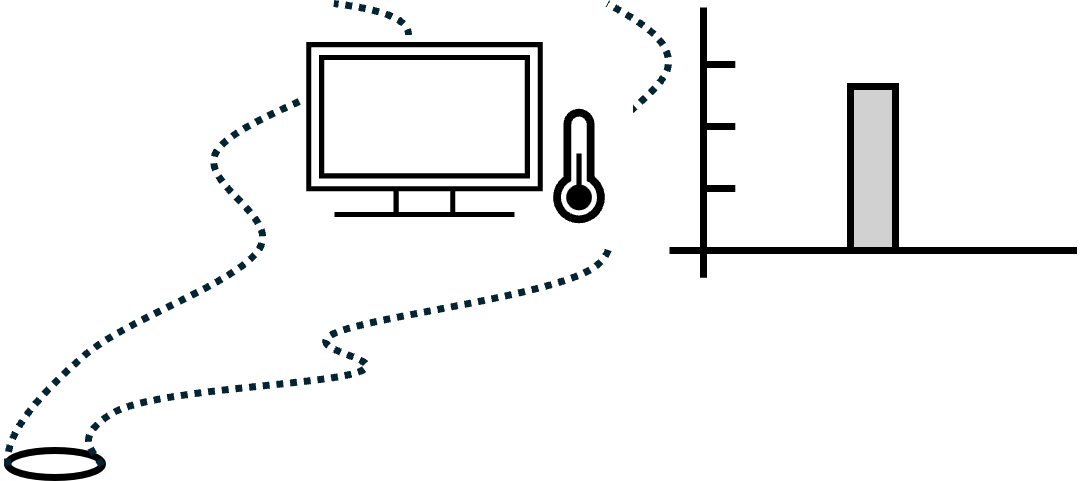
\includegraphics{fig/gassensor.png}
    \caption{電気化学式センサによる火山ガス観測イメージ}
    \label{fig:gassensor_image}
\end{figure}

これらの課題に対し, 微量気体を遠隔かつ空間分布, 
さらに時間連続的に観測する手法として, 
差分吸収ライダー（DIAL: Differential Absorption Lidar）
の利用が期待されている. 
DIALは, 測定対象気体に対して吸収特性の異なる2波長のレーザを照射し, 
その受信信号の差から濃度分布を推定する手法である. 
電気化学式センサと比較して, 
遠隔から周辺領域の濃度分布を時間的に連続して測定可能である点において優れている.

\begin{figure}
    \centering
    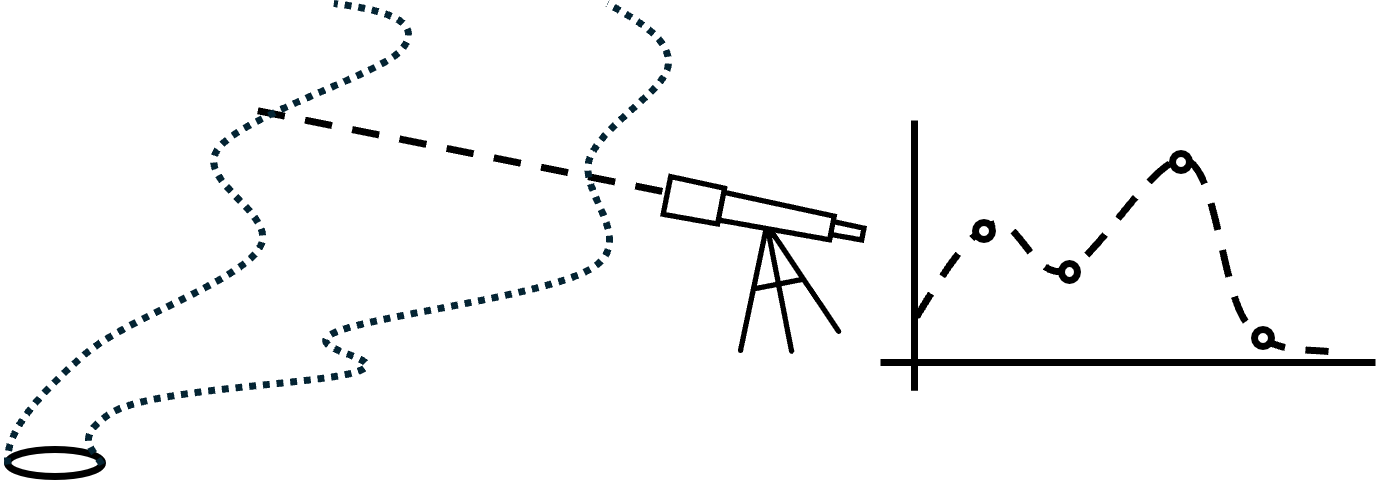
\includegraphics{fig/lidar.png}
    \caption{ライダーによる火山ガス観測イメージ}
    \label{fig:lidar_image}
\end{figure}

\newpage
\section{ラマンDIAL}
本研究で提案するラマンDIALは, 送信するレーザ波長によって生じる
ラマン散乱光をシステムに用いる受信波長として構成し, 
気体濃度の分布を測定する手法である. 
ラマン散乱とは, 
入射したレーザ光が分子の振動エネルギー準位と相互作用することで, 
入射光とは異なる波長成分を持つ散乱光が生成される現象である.
また, ラマン散乱には長波長側にシフトするストークス散乱と, 
短波長側にシフトするアンチストークス散乱が存在し, 
一般的にアンチストークス散乱の強度はストークス散乱と比較して 
1/10 以下と非常に微弱である. 
\cref{fig:ramanDIAL}にラマンDIALの基本的な構成を示す. 
\begin{figure}
    \centering
    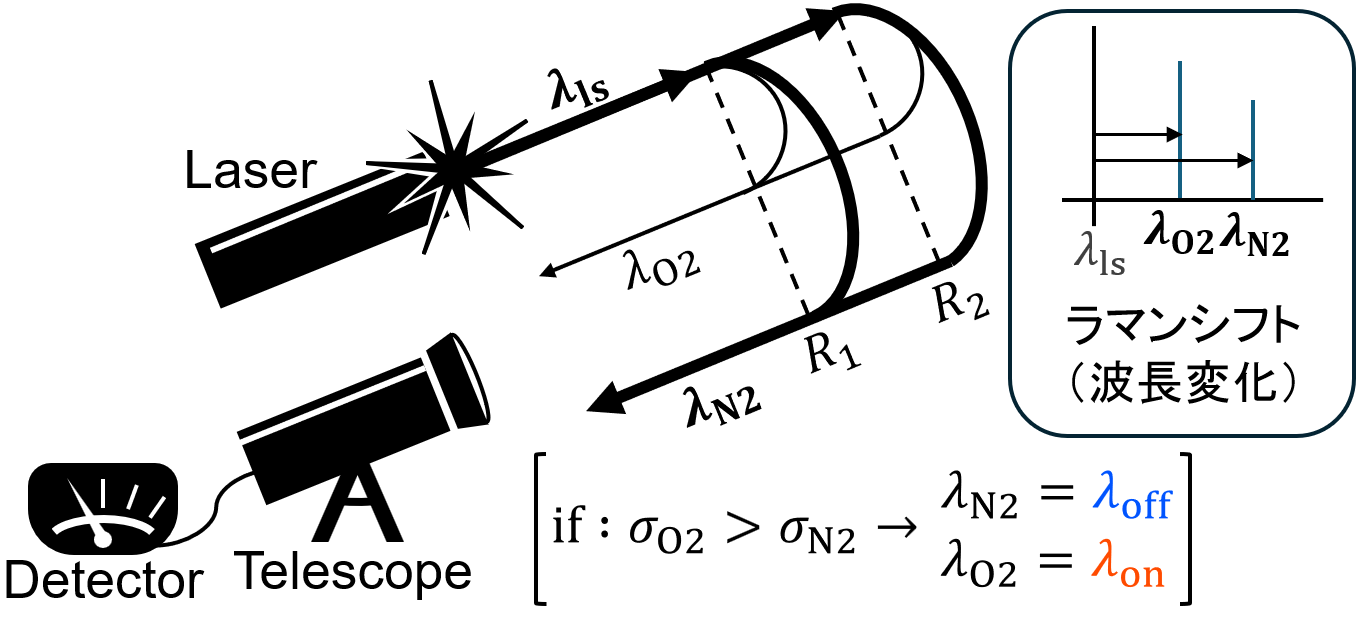
\includegraphics[width=0.8\linewidth]{fig/ramanDIAL.png}
    \caption{ラマンDIAL構成図}
    \label{fig:ramanDIAL}
\end{figure}

\noindent
今回提案するラマンDIALは大気中の酸素分子（\ce{O2}）及び窒素分子(\ce{N2})のラマン散乱を利用する. 
\ce{O2}のラマンシフトは\qty{1556}{cm^{-1}}, 
\ce{N2}のラマンシフトは\qty{2331}{cm^{-1}}であり, 
それぞれのラマン散乱波長はレーザ波長に対して, 
このラマンシフト分だけ波長変化することになる. 
ここで, 対象気体の吸収が強い波長をオン波長\subrm{\lambda}{on}, 
吸収が弱い波長をオフ波長\subrm{\lambda}{off}と呼ぶ. 
この手法の特徴は, 通常のDIALに対して, 送信レーザの波長数を削減し, 
受信側で2波長を構成できることであり, 
これによりシステムの小型化が期待される.

\newpage
ライダー視線上の距離$R$におけるライダーの受信光子数\subrm{P}{phot}は
\cref{equ:power,equ:alpha}で求められる\cite{PowerEqu}. 
\begin{align}
    P(R)
    &=\frac{E_0}{h\subrm{\lambda}{ls}}
    M \eta q \Delta R \frac{A}{R^2}O(R) \subrm{\beta}{ram}
    \exp\ab[
        \int^{R}_{0}
            \ab(
                \alpha(r, \subrm{\lambda}{ls})
                +\alpha(r, \subrm{\lambda}{ram})
            )\dd r 
    ]\label{equ:power}\\
    \alpha(\lambda, r) 
    &= \subrm{\alpha}{air}(\lambda)
    +\sum^{N}_{\mathrm{gas}=1}
        \subrm{n}{gas}(r)\subrm{\sigma}{gas}(\lambda)\label{equ:alpha}
\end{align}

\noindent
式中の$E_0$はパルスエネルギー, 
$h$はプランク定数, 
$M$は積算回数, 
$q$は光学系の全効率, 
$\eta$はディテクターの量子効率, 
$\Delta R$は距離分解能, 
$A$は受信鏡直径
$O(R)$は重なり関数を表す. 
後方ラマン散乱断面積\subrm{\beta}{ram}について,
清水らが報告した結果から, 
窒素の\subrm{\beta}{ram}は\qty{2.8e-34}{m^2}, 
酸素の\subrm{\beta}{ram}は\qty{3.9e-34}{m^2}とした\cite{ramanXS}. 
そして, これを0.1した値をアンチストークス散乱の後方散乱断面積とした. 
% 式中の$C$はライダーのシステムパラメータ, 
% $\beta_{ram}$は後方ラマン散乱断面積,  
% $\lambda_{\mathrm{ls}}$はレーザ波長, 
% $\lambda_{\mathrm{ram}}$はラマン散乱波長である.  
\cref{equ:alpha}に示す消散係数$\alpha$は, 大気及び各種気体による吸収の総和であり, 
ここでgas=1,2,…,Nはガス成分の種類を表す. 

距離$R_1, R_2(R_1<R_2)$における2波長\subrm{\lambda}{on}, 
\subrm{\lambda}{off}のライダーの受信光子数から\ce{SO2}の濃度分布は
\cref{equ:n_SO2}で求められる\cite{DIALEqu}.
\Delta\sigma はon波長とoff波長における
\ce{SO2}吸収断面積の差分である. 
\begin{equation}
    \subrm{n}{SO2}
    =\frac{1}{\Delta\subrm{\sigma}{SO2}\Delta R}\ln\ab(
        \frac
        {P(\subrm{\lambda}{on}, R_1)P(\subrm{\lambda}{off}, R_2)}
        {P(\subrm{\lambda}{on}, R_2)P(\subrm{\lambda}{off}, R_1)}
    )\label{equ:n_SO2}
    % \Delta\sigma_{\mathrm{SO2}} &= 
    % \sigma_{\mathrm{SO2}}(\lambda_{\mathrm{on}})-
    % \sigma_{\mathrm{SO2}}(\lambda_{\mathrm{off}})
\end{equation}

% \begin{table}[t]
%   \centering
%   \caption{System parameters for Raman DIAL.}
%   \label{tab:system_parameters}
%   \begin{tabular}{c p{60mm} p{20mm}}
%     \hline
%     $E_0$ [mJ] & Pulse energy & 30 \\
%     $A$ [m] & Diameter of the telescope & 0.6 \\
%     $M$ & Number of integration times & $100 \si{Hz}\times$30 \si{min} \\
%     $\eta$ & Quantum efficiency of the detector & 0.3 \\
%     $q$ & Total efficiency of optics & 0.3 \\
%     $\Delta R$ [m] & Spatial resolution & 30 \\

%     % $\sigma_{\mathrm{RamanN2}}$ [m$^2$] &
%     % Stokes Raman scattering cross section of N$_2$ &
%     % $2.8 \times 10^{-34}$ \\

%     % $\sigma_{\mathrm{RamanO2}}$ [m$^2$] &
%     % Stokes Raman scattering cross section of O$_2$ &
%     % $3.9 \times 10^{-34}$ \\

%     % $\sigma'_{\mathrm{ramN2}}$ [m$^2$] &
%     % anti-Stokes Raman scattering cross section of N$_2$ &
%     % $2.8 \times 10^{-35}$ \\

%     % $\sigma'_{\mathrm{ramO2}}$ [m$^2$] &
%     % anti-Stokes Raman scattering cross section of O$_2$ &
%     % $3.9 \times 10^{-35}$ \\
%     \hline
%   \end{tabular}
% \end{table}

\section{本研究の目的}
本研究は, ラマンDIALの遠隔・分布・時間的連続観測に着目し, 
火山ガス中の\ce{SO2}の測定への適応可能性を数値シミュレーションにより
検証することを目的とする.
目安として, \ce{SO2}濃度に対する±\qty{10}{\%}の測定誤差を基準に設定した. 

本研究の新規性として, 
信号強度の課題からこれまで十分検討されてこなかった
アンチストークス散乱信号に注目し, 
アンチストークス散乱波長を含む受信波長構成と
従来構成を定量的に比較した点が挙げられる. 

\chapter{レーザ波長および受信波長構成の最適条件の検討}\label{chapt2}

本章では, ラマンDIALによる二酸化硫黄分布観測を対象として,
統計誤差および干渉誤差の波長依存性を数値シミュレーションにより評価し,
レーザ波長および受信波長構成の最適条件について検討した. 

\section{ラマンDIALの統計誤差}
ラマンDIALによる測定で発生する統計誤差は
\cref{equ:stat_err}で求められる\cite{StatErrorEqu}. 
式中の$D$はダークカウント, $B_j$は背景光雑音, 
$F$はディテクターの雑音指数を表す. 
$\mathrm{i}=1,2$ はon波長及びoff波長,  
$\mathrm{j}=1,2$ は視線距離$R_1, R_2$に相当する. 
\begin{align}
    \staterr 
    &= \dfrac{1}{2\Delta\subrm{\sigma}{SO2} \Delta R}\ab[
        \sum^2_{i=1}\sum^2_{j=1}
        \frac{D+(P_{ij}+B_j)F}{P_{ij}}
    ]^{1/2}
    \label{equ:stat_err}
\end{align}

\cref{equ:stat_err}より, 
統計誤差\staterr はレーザ波長$\subrm{\lambda}{ls}$に依存し, 
依存関係は\cref{fig:staterr_dep}に表せる. 

\begin{figure}
\centering
\begin{tikzpicture}[
    mynode/.style={
        draw, 
        rectangle, 
        rounded corners, 
        minimum width=4cm, 
        minimum height=1cm,
        align=center
    }
]
    % 各段のY座標（等間隔）
    \def\first{0}      % 1段目：レーザ波長
    \def\second{-2}     % 2段目：ラマン散乱波長
    \def\third{-4}     % 3段目：PとΔσ
    \def\fourth{-6}     % 4段目：統計誤差

    % ノード定義
    \node[mynode, fill=blue!15] (lambda_ls) at (0,\first) {レーザ波長 $\subrm{\lambda}{ls}$};
    \node[mynode] (lambda_ram) at (0,\second) {ラマン散乱波長 $\subrm{\lambda}{ram}$};
    \node[mynode] (P) at (-3,\third) {受信光子数 $P$};
    \node[mynode] (dxs) at (3,\third) {\ce{SO2}差分吸収断面積 $\Delta\subrm{\sigma}{SO2}$};
    \node[mynode, fill=red!20] (staterr) at (0,\fourth) {統計誤差 $\staterr$};

    % 矢印
    \draw[->, thick] (lambda_ram) -- (lambda_ls) node[midway, left] {依存};
    \draw[->, thick] (P) -- (lambda_ram);
    \draw[->, thick] (dxs) -- (lambda_ram);
    \draw[->, thick] (staterr) -- (P);
    \draw[->, thick] (staterr) -- (dxs);
\end{tikzpicture}
\caption{ラマンDIALにおけるレーザ波長$\subrm{\lambda}{ls}$と統計誤差 $\staterr$ の依存関係}
\label{fig:staterr_dep}
\end{figure}

\noindent
\ce{SO2}吸収が強すぎる
ラマン散乱波長$\subrm{\lambda}{ram}$
で$P$は小さくなる一方で, 
\ce{SO2}吸収が弱すぎる
on波長$\subrm{\lambda}{on}(=\subrm{\lambda}{ram})$
で$\dxs$は小さくなり, 
いずれも\staterr が増大するため, 
それぞれのバランスが肝要となる. 
すなわち, ラマンDIALには
$P$と$\dxs$が十分大きく, 
\staterr が最小となる$\subrm{\lambda}{ls}$が存在する. 

\newpage
二酸化硫黄（\ce{SO2}）, 
オゾン（\ce{O3}）, 
硫化水素（\ce{H2S}）の吸収スペクトルを\cref{fig:3gases_absorption}に示す. 
縦軸は消散係数（= $\subrm{n}{gas}(R)\times\subrm{\sigma}{gas}(\lambda)$）である. 
吸収断面積のデータセットはThe MPI-Mains UV/VIS Spectral Atlasより取得し, 
吸収スペクトルは各気体の濃度による数密度と吸収断面積を乗じた消散係数である. 
\cite{
MPI_Mainz_UV_VIS_Atlas2013,
SO2_dataset_Hermans2009_I,
SO2_dataset_Vandaele2009_II,
O3_dataset_Bogumil2003,
H2S_dataset_Grosch2015,
}.

\begin{figure}
    \centering
    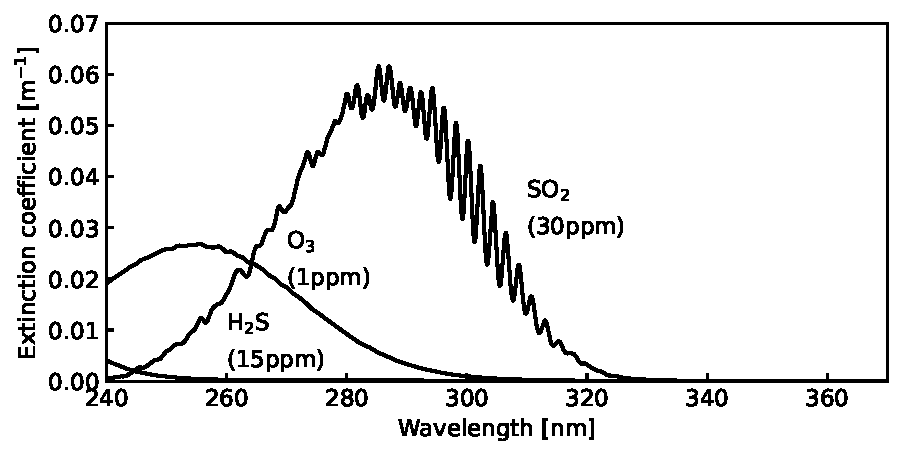
\includegraphics{fig/sim_01_3gases_absorp}
    \caption{\ce{SO2}, \ce{O3}, \ce{H2S}の吸収スペクトル}
    \label{fig:3gases_absorption}
\end{figure}
\noindent
二酸化硫黄は紫外領域に吸収スペクトルを持ち, 
300 nm 付近の波長では吸収が櫛状に増減する特徴を持つ. 
二酸化硫黄測定にラマン DIALを適応する場合, 
\staterr は, これらの吸収スペクトルに依存する. 
改めて, \cref{equ:stat_err}の 
$P$ と $\Delta\subrm{\sigma}{SO2}$はon波長とoff波長に依存し, 
on波長及びoff波長に相当するラマン散乱波長はレーザ波長に依存する. 
したがって, \ce{SO2}測定のためのラマンDIALは, 
火山ガスの吸収スペクトル形状に合わせて,
受信強度と差分吸収が十分に確保できるレーザ波長の最適点が存在する.

\newpage
そして, 受信するon波長とoff波長の構成にも注意する必要がある. 
ラマン散乱におけるレーザ波長\subrm{\lambda}{ls}と
ラマン散乱波長\subrm{\lambda}{ram}, 
ラマンシフト\subrm{\lambda}{shift}の関係は\cref{fig:raman_shift}に示すとおりである. 

\begin{figure}
    \centering
    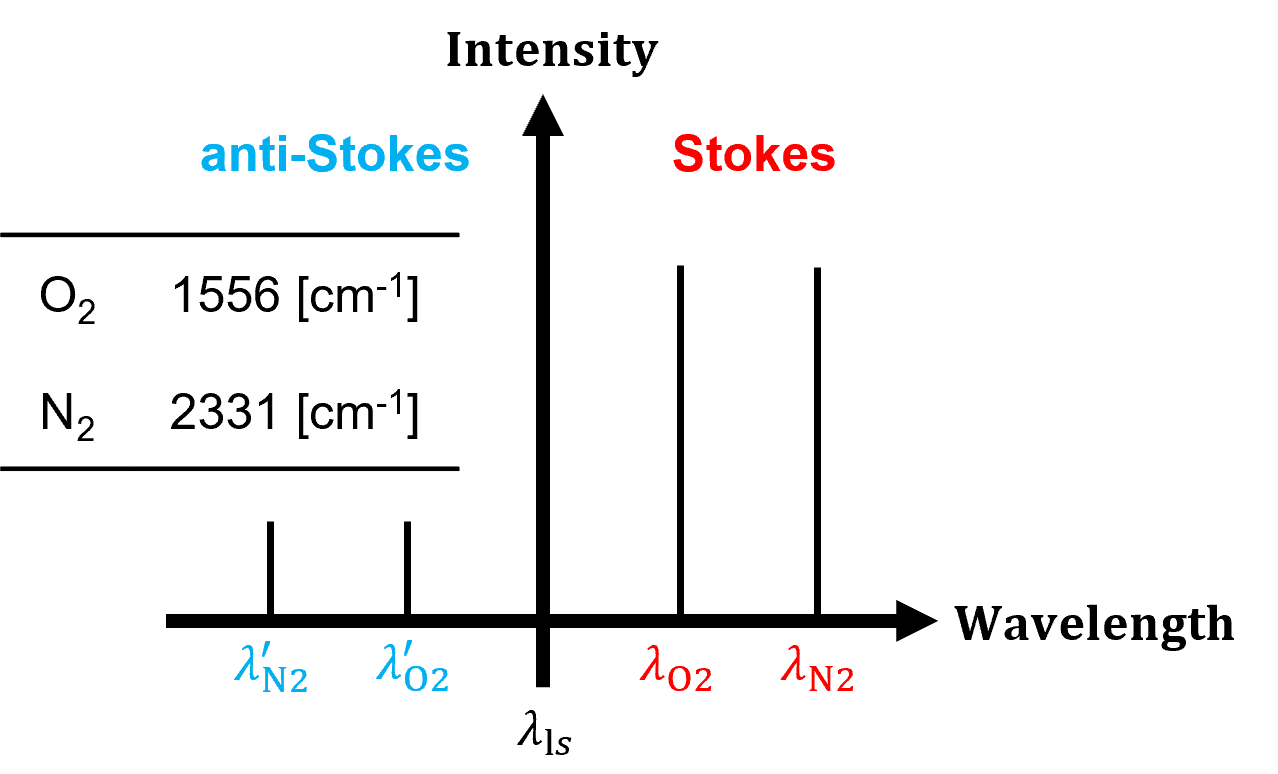
\includegraphics{fig/raman_stokes_Astokes}
    \caption{レーザ波長とラマン散乱波長の関係}
    \label{fig:raman_shift}
\end{figure}

\noindent
酸素分子\ce{O2}によるラマン散乱波長には,
ストークス散乱波長$\subrm{\lambda}{O2}$と
アンチストークス散乱波長$\subrm{\lambda}{O2}'$の2種類が存在し,
窒素分子\ce{N2}についても同様である.
そのため,1つのレーザ波長からラマンDIALの受信波長を構成する場合, 
\ce{O2} および \ce{N2} のストークス・アンチストークス散乱を含む
計 4 つのラマン散乱波長から on 波長および off 波長を選択可能であり,
その組合せは 6 通りとなる.

一般に,アンチストークス散乱はストークス散乱と比較して信号強度が弱く,
ラマンDIALをはじめとしたラマン散乱を利用する測定系では, 
アンチストークス散乱波長は実用上利用されにくい.
そのため,先行研究では Nd:YAG レーザの第 4 高調波である \qty{266}{nm} に対し,
酸素および窒素のストークス散乱波長のみを用いた
ラマンDIAL測定系について検討した\cite{Previous_research}.

しかし, アンチストークス散乱波長が受信波長として利用可能であるとすれば,
従来法の受信波長構成に加えて,新たに 5 つの受信波長構成が検討対象となる.
これら 6 つの受信波長構成は, 
同じレーザ波長でも on 波長および off 波長の波長配置がそれぞれ異なるため,
それに依存する統計誤差 $\staterr$ も異なる.
したがって, その中でも統計誤差が小さい最適な受信波長構成が存在する.

本章では, 6つの受信波長構成で統計誤差を計算し, 比較した結果を示す.
6つの受信波長構成それぞれで最適レーザ波長のときの統計誤差を比較し, 
最も小さいものを最適な受信波長構成とする. 

\newpage
\section{シミュレーション条件}
高度$z$, 波長$\lambda$, ライダー視線距離$R$における大気モデルは以下の通りとした. 
\cref{equ:atmnumber}は大気密度, 
\cref{equ:sigmaray}はレイリー散乱断面積, 
\cref{equ:betamol}は大気分子の後方散乱係数,
\cref{equ:aermodel}エアロゾルモデル, 
\cref{equ:betaaer}はエアロゾルの後方散乱係数, 
\cref{equ:alphamol}は大気分子の消散係数, 
\cref{equ:alphaaer}はエアロゾルの消散係数, 
\cref{equ:alphagas}は光路上の気体の消散係数（$i=1,2,...,N$はN個のガス種）を表す.
\begin{align}
    &N(z)
    =2.60\times10^{25}\exp\left(
        -1.08\times10^{-4}z
    \right)&[\si{m^{-3}}]
    \label{equ:atmnumber}\\
    &\subrm{\sigma}{ray}(\lambda)
    =5.45\times10^{-32}\left(\frac{550}{\lambda}\right)&[\si{m^{2}}]
    \label{equ:sigmaray}\\
    &\subrm{\beta}{mol}(z, \lambda)
    =N(z)\subrm{\sigma}{ray}(\lambda)&[\si{m^{-1}}]
    \label{equ:betamol}\\
    &\subrm{M}{aer}(z, \lambda)
    =36.31\exp(-.78\times10^{-4}\subrm{\beta}{mol}(z))\left(\frac{\lambda}{710}\right)^4
    \label{equ:aermodel}\\
    &\subrm{\beta}{aer}(z, \lambda)
    =\subrm{M}{aer}(z, \lambda)\times\left(\frac{710}{\lambda}\right)&[\si{m^{-1}}]
    \label{equ:betaaer}\\
    &\subrm{\alpha}{mol}=\frac{8\pi}{3}\subrm{\beta}{mol}&[\si{m^{-1}}]
    \label{equ:alphamol}\\
    &\subrm{\alpha}{aer}(z)
    =s\subrm{\beta}{aer}(z)&[\si{m^{-1}}]
    \label{equ:alphaaer}\\
    &\subrm{\alpha}{gas}(z, R, \lambda)
    =\sigma_{i=1}^{N}\subrm{N}{gas}(z, R)\subrm{\sigma}{gas}(\lambda)&[\si{m^{-1}}]
    \label{equ:alphagas}
\end{align}

\cref{fig:gas_setting}に, シミュレーションに用いる火山ガス濃度分布の設定値を示す. 
設定値を決めるにあたって, 三宅島での観測データを参考にした\cite{miyake}.
地表面の火口から二酸化硫黄を含む火山ガスが噴出している環境を想定し, 
高度\qty{1}{km}地点の水平\qty{1}{km}を観測領域に設定した. 
観測領域内の\qty{300}{m}から\qty{700}{m}を火山ガスが濃厚な高濃度区間, 
それ以外を火口から遠い低濃度区間とした. 
気温について, 低濃度区間は\qty{298}{K}, 
高濃度区間は\qty{358}{K}を想定した. 
これは放出される高温の火山ガスがある程度拡散した状況を想定しており, 
気温は用いる吸収断面積のデータセットに反映されている. 
三宅火山は, 近年\ce{SO2}放出量が減少傾向で,
2016年頃から1日あたりの放出量が数十トン以下と少なくなっているが,
三宅空港での監視データでは,
2001年2月から3月末までの2ヶ月間の間に最大で約\qty{11}{ppm}の高濃度が観測されており, 
風による移流の影響を加味すると火口付近はさらに高濃度であると推測される.
そのため, 高濃度区間は二酸化硫黄が\qty{30}{ppm},
硫化水素が\qty{15}{ppm}とし, 
低濃度区間は二酸化硫黄は\qty{0.07}{ppm}
硫化水素は\qty{0.035}{ppm}に設定した. 
オゾンは観測領域全体で一定の\qty{0.005}{ppm}とした. 

\begin{figure}
    \centering
    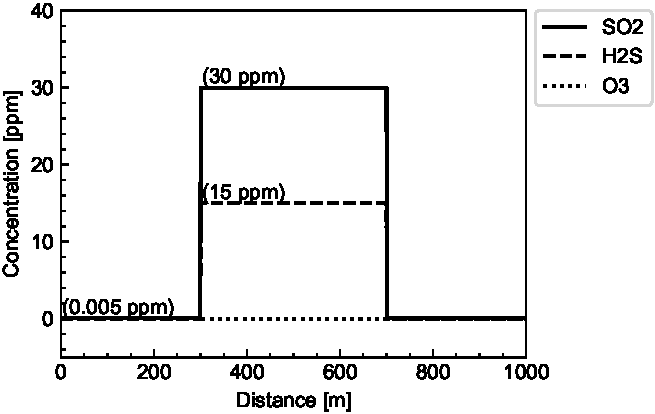
\includegraphics{fig/sim_01_env_LoS}
    \caption{火山ガス濃度分布の設定}
    \label{fig:gas_setting}
\end{figure}

\newpage
\cref{equ:power}及び\cref{equ:stat_err}で用いる
システムパラメータは\cref{tab:sys_params}に示すとおりである.
\begin{table}
    \centering
    \caption{システムパラメータ設定値}
    \label{tab:sys_params}
    \begin{tabular}{lcc}
        \hline
        \hline
        Pluse energy                &$E_0$                      & \qty{10}{mJ} \\
        Laser repetition frequency  &$f$                        & \qty{100}{Hz} \\
        Integration time            &$\subrm{t}{m}$             & \qty{10}{min} \\
        Number of integrations      &$M=f\times \subrm{t}{m}$   & \num{6.0e4}\\
        Receiver telescope diameter &$A$                        & \qty{0.3}{m} \\
        Total optical efficiency    &$q$                        & 0.3 \\
        Detector quantum efficiency &$\eta$                     & 0.3 \\
        Spatial resolution          &$\Delta R$                 & \qty{5}{m} \\
        Dark counts                 &$D$                        & 0\\
        Background light noise      &$B$                        & 0\\
        Detector noise factor       &$F$                        & 1 \\
        \hline
        \hline
    \end{tabular}
\end{table}

\noindent
ラマンDIALによる観測の特徴である時間連続性は積算時間を10 分としており, 
分布観測性は距離分解能を\qty{5}{m}としている. 
すなわち得られる測定データは10分間の時間平均, 
\qty{5}{m}区間の距離平均濃度を意味する. 
また, 本研究全体を通して, 
背景光雑音及びダークカウント, ディテクター雑音指数による影響を
無視した理想条件でシミュレーションした. 

\newpage
\section{受信波長の構成による統計誤差の比較}
\cref{fig:raman_shift}に示したように, 
レーザ波長によって生じるラマン散乱波長は4つあり, 
それらから受信する2波長を選択するとき取り得る構成は6通りとなる. 
それぞれで, \staterr が最小となるレーザ波長を探索し, 
そのときの\staterr の距離特性を比較することで最適な受信波長の構成を決定する.
\cref{fig:6combies_stat}に, 
各受信波長の構成における統計誤差を示す.
\begin{figure}
    \centering
    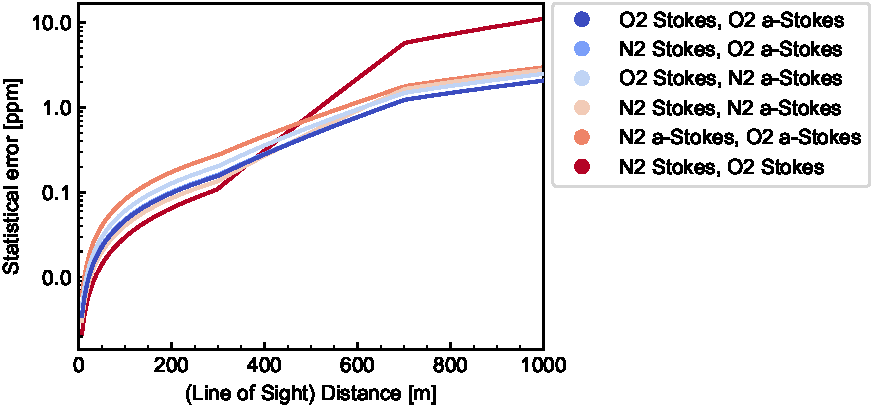
\includegraphics{fig/sim_01_6combies_stat}
    \caption{受信波長の構成による統計誤差の比較}
    \label{fig:6combies_stat}
\end{figure}

\noindent
横軸はライダーの視線距離, 
縦軸は\ce{SO2}測定値に対する統計誤差を表し, 
単位はそれぞれ\unit{m}, \unit{ppm}である. 
それぞれの最適レーザ波長は, 
高濃度区間（\qty{300}{m}から\qty{700}{m}）で最遠方測定点となる
\qty{700}{m}の少し手前を基準に最も統計誤差が最小となるものを選択した.
\ce{N2}ストークス散乱波長と\ce{O2}ストークス散乱波長の構成は, 
視線距離で近傍の低濃度区間では優位であるものの, 
高濃度区間での悪化が激しく, 
観測領域終端では\qty{10}{ppm}を超過した. 
反対に, 
\ce{O2}ストークス散乱波長と\ce{O2}アンチストークス散乱波長の構成は, 
統計誤差の距離悪化が緩やかで, 
その他の構成と比較しても統計誤差が小さかった. 

6つの組み合わせそれぞれの最適レーザ波長とオン波長, オフ波長, 
そして基準点での統計誤差を\cref{tab:6combies_3wlandstaterr}に示す. 
レーザ波長に注目すると, 
\ce{N2}ストークス散乱波長と\ce{O2}ストークス散乱波長の構成は
最適レーザ波長が\qty{240}{nm}で, 
それ以外の構成では\qty{340}{nm}前後となっている.
\cref{fig:3gases_absorption}に示したように, 
波長\qty{240}{nm}付近は\ce{H2S}吸収が存在するため統計誤差が悪化しやすい. 
また, それ以降の波長でも\ce{SO2}, 
\ce{O3}ともに吸収が強くなるため同様に統計誤差が悪化しやすい. 
そのため, 紫外領域となる\ce{340}{nm}付近に最適レーザ波長が集まったと考えられる. 
そして, \staterr に注目すると, 
\ce{SO2}濃度の設定値\qty{30}{ppm}に対して, 
\ce{N2}ストークス散乱波長と\ce{O2}ストークス散乱波長の構成では
\staterr は\qty{5}{ppm}以上であり, 設定値の10\%を超過している. 
しかし, それ以外の構成では1\sim 2\unit{ppm}と数\%であるため, 
これらの組み合わせは今回の条件下において, 
\ce{SO2}測定に適する構成である. 
\begin{table}
    \centering
    \caption{各受信信号構成の最適レーザ波長と受信波長, 統計誤差}
    \label{tab:6combies_3wlandstaterr}
    \begin{tabular}{ccccc}
        \hline
        Combi.  
        & Laser wavelength[\unit{nm}] 
        & \subrm{\lambda}{on}[\unit{nm}] 
        & \subrm{\lambda}{off}[\unit{nm}] 
        & \staterr [\unit{ppm}]\\

        \ce{O2} Stokes, \ce{O2} a-Stokes
        & 334.6
        & 318.0
        & 353.0
        & 1.21\\

        \ce{N2} Stokes, \ce{O2} a-Stokes
        & 334.6
        & 318.0
        & 362.9
        & 1.22\\

        \ce{O2} Stokes, \ce{N2} a-Stokes
        & 343.7
        & 318.2
        & 362.1
        & 1.47\\

        \ce{N2} Stokes, \ce{N2} a-Stokes
        & 338.9
        & 314.1
        & 368.0
        & 1.61\\

        \ce{N2} a-Stokes, \ce{O2} a-Stokes
        & 343.6
        & 318.1
        & 326.1
        & 1.75\\

        \ce{N2} Stokes, \ce{O2} Stokes
        & 240.0
        & 254.2
        & 249.3
        & 5.56\\






        \hline
    \end{tabular}
\end{table}

さらに, 統計誤差の距離特性が劣っていた
\ce{N2}ストークス散乱波長と\ce{O2}ストークス散乱波長の構成と, 
統計誤差の距離特性が優れた
\ce{O2}ストークス散乱波長と\ce{O2}アンチストークス散乱波長の構成に注目する. 
\cref{fig:6combies_stat}に2つの受信波長構成それぞれのレーザ波長, 
on波長及びoff波長における吸収断面積を示す. 
横軸は波長, 縦軸は吸収断面積である. 
\begin{figure}
    \centering
    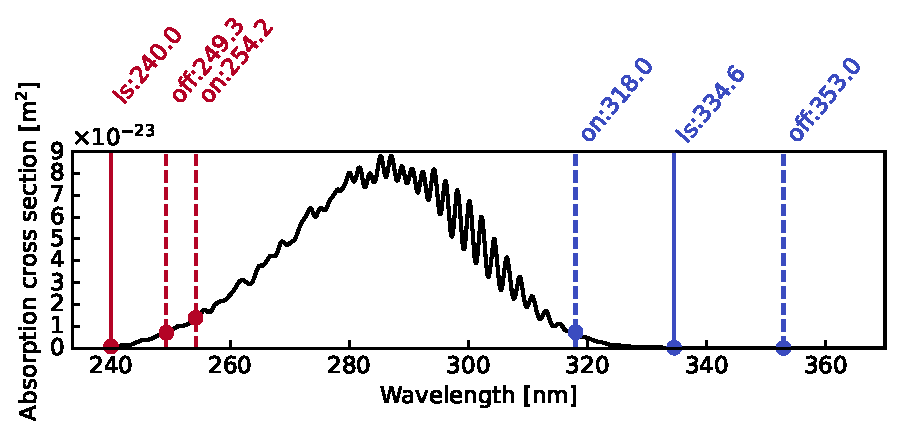
\includegraphics{fig/sim_01_cond_2case}
    \caption{二つの受信波長構成（\ce{N2}ストークス散乱波長と\ce{O2}ストークス散乱波長, 
        \ce{O2}ストークス散乱波長と\ce{O2}アンチストークス散乱波長）における\ce{SO2}吸収断面積}
    \label{fig:cond_wl_combi}
\end{figure}

\noindent
どちらもレーザ波長は山なりの吸収スペクトルから外れており, 
on波長, off波長それぞれの吸収断面積は, 
\ce{N2}ストークス散乱波長と\ce{O2}ストークス散乱波長の構成の方が大きい. 
また, \Delta \subrm{\sigma}{SO2}は, 
\ce{N2}ストークス散乱波長と\ce{O2}ストークス散乱波長の受信構成で\qty{6.83e-24}{m^2}, 
\ce{O2}ストークス散乱波長と\ce{O2}アンチストークス散乱波長の受信構成で\qty{7.22e-24}{m^2}であり, 
僅かに\ce{O2}ストークス散乱波長と\ce{O2}アンチストークス散乱波長の受信構成の方が大きい. 

\cref{fig:cond_power_combi}は, 
\ce{N2}ストークス散乱波長と\ce{O2}ストークス散乱波長の構成と, 
\ce{O2}ストークス散乱波長と\ce{O2}アンチストークス散乱波長の構成における
on波長及びoff波長の信号強度の距離特性であり, 縦軸は受信光子数である. 
\begin{figure}
    \centering
    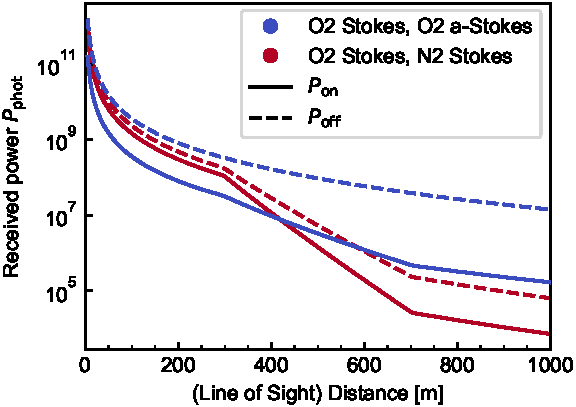
\includegraphics{fig/sim_01_power}
    \caption{
        二つの受信波長構成（\ce{N2}ストークス散乱波長と\ce{O2}ストークス散乱波長, 
        \ce{O2}ストークス散乱波長と\ce{O2}アンチストークス）における受信光子数の距離特性
    }
    \label{fig:cond_power_combi}
\end{figure}

\noindent
赤色で示す\ce{O2}ストークス散乱波長と\ce{N2}ストークス散乱波長の受信波長構成において, 
実線は\ce{N2}ストークス散乱信号（$\subrm{\lambda}{on}=\qty{254.2}{nm}$）, 
点線は\ce{O2}ストークス散乱信号（$\subrm{\lambda}{off}=\qty{249.3}{nm}$）である. 
青色で示す\ce{O2}ストークス散乱波長と\ce{O2}アンチストークス散乱波長の受信波長構成において,
実線は\ce{O2}アンチストークス散乱信号（$\subrm{\lambda}{on}=\qty{318.0}{nm}$）, 
点線は\ce{O2}ストークス散乱信号（$\subrm{\lambda}{off}=\qty{353.0}{nm}$）である. 

\newpage
高濃度の\ce{SO2}による吸収を受ける\qty{300}{m}以前の信号強度を比較すると, 
\cref{equ:power}を解く際に
アンチストークス散乱の信号強度は
ストークス散乱のものに対して1/10となるよう計算したため, 
青実線で示す\ce{O2}アンチストークス散乱は他の3つと比べて小さい.
また, on波長同士では赤色実線で示す\ce{N2}ストークス散乱波長の方が強く, 
off波長同士では青色点線で示す\ce{O2}ストークス散乱波長の方が強い. 
一方で, \qty{700}{m}地点の信号強度を比較すると, 
on波長, off波長どちらも青色で示す
\ce{O2}アンチストークス散乱波長, 
\ce{O2}ストークス散乱波長の方が強い. 
2つの受信構成の$\Delta \subrm{\sigma}{SO2}$は同程度であるため, 
$\subrm{P}{on}, \subrm{P}{off}$が大きい方が
\staterr は小さくなる. 
したがって, 
\ce{O2}アンチストークス散乱波長$\subrm{\lambda}{on}=\qty{318.0}{nm}$の信号強度は
近傍で弱かったものの, 
\ce{SO2}吸収が弱いために信号減衰が小さく, 
遠方での統計誤差に優れた. 

\newpage
\section{ラマンDIALによる二酸化硫黄測定における干渉誤差}
ラマンDIALにおいて測定対象でない物質による吸収は, 
干渉誤差（オフセット誤差）を発生させる. 
火山環境において, 大気や火山ガス中には二酸化硫黄以外にも紫外域に吸収を持つ気体
（オゾンや硫化水素）が存在するため,
それらによる吸収は干渉誤差を引き起こす. 
\cref{equ:contam_err}は干渉要素を補正するための項であり, 
対象気体濃度を算出するためにDIAL方程式を解く際に,
あらかじめ干渉要素の推定値を含めることで 
その影響をある程度補正することが可能である. 
\begin{align}
    \cntmerr
    &= \frac{\Delta \subrm{\alpha}{air}
    +\Sigma^N_{\mathrm{gas}=1}\subrm{n}{gas}\Delta\subrm{\sigma}{gas}}{\Delta \subrm{\sigma}{SO2}}\label{equ:contam_err}
\end{align}
gas=1,2,...,Nは測定時に推定するガス種を表す. 
例えば, オゾンによる干渉を補正したい場合, 
オゾンのおおよその濃度\subrm{n}{O3}を推定し, 
on波長とoff波長における二酸化硫黄, オゾンの差分吸収断面積\subrm{\sigma}{SO2}, \subrm{\sigma}{O3}を
を用意して
\subrm{n}{O3}\times\Delta\subrm{\sigma}{O3}/\Delta\subrm{\sigma}{SO2}
を計算する. これを\cref{equ:n_SO2}から引くことで
補正後の二酸化硫黄濃度の推定値が得られる.
このとき, 推定した濃度が実際の濃度と異なる場合,
干渉誤差が残存することになる.

測定する火山ガス濃度は, 
その火山の熱水系構造や活動状況によって放出量は異なり, 
また, 火口からの距離などによって移流や拡散を伴って濃度は変動する.
そのため, 二酸化硫黄放出が微量であったり, 
それ以外の干渉気体が豊富であったりという
二酸化硫黄の相対量が少ない環境での測定を考えると, 
干渉誤差の影響は無視できないため, 
統計誤差と同様に考慮する必要がある.

\newpage
\cref{fig:6combies_cntm}に各受信波長の構成における干渉誤差を示す. 
横軸はライダーの視線距離, 
縦軸は\ce{SO2}濃度の測定値である. 
\cref{tab:6combies_cntmerr}は低濃度区間にあたる視線距離\qty{100}{m}と
高濃度区間にあたる視線距離\qty{500}{m}における
各受信波長構成の干渉誤差である.

\begin{figure}
    \centering
    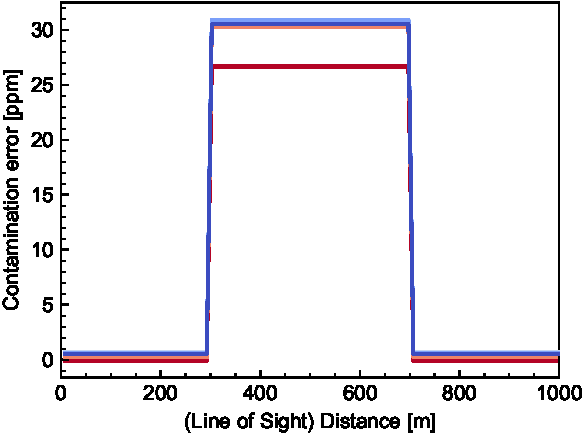
\includegraphics{fig/sim_01_6combies_cntm}
    \caption{受信波長の構成による干渉誤差の比較}
    \label{fig:6combies_cntm}
\end{figure}

\begin{table}
    \centering
    \caption{各受信波長構成の近傍（\qty{100}{m}）及び遠方（\qty{500}{m}）における干渉誤差}
    \label{tab:6combies_cntmerr}
    \begin{tabular}{ccc}
        \hline
        Combi.  
        & \cntmerr(R=100) [\unit{ppm}] 
        & \cntmerr(R=500) [\unit{ppm}] \\

        \ce{O2} Stokes, \ce{O2} a-Stokes
        & 0.47
        & 0.51\\

        \ce{N2} Stokes, \ce{O2} a-Stokes
        & 0.57
        & 0.89\\

        \ce{O2} Stokes, \ce{N2} a-Stokes
        & 0.61
        & 0.93\\

        \ce{N2} Stokes, \ce{N2} a-Stokes
        & 0.48
        & 0.89\\

        \ce{N2} a-Stokes, \ce{O2} a-Stokes
        & 0.14
        & 0.29\\

        \ce{N2} Stokes, \ce{O2} Stokes
        & -0.17
        & -3.32\\
        \hline
    \end{tabular}
\end{table}

\noindent
\ce{N2}ストークス散乱波長と\ce{O2}ストークス散乱波長の構成での
高濃度区間の干渉誤差が\qty{-3.32}{ppm}と最も大きく, 
それ以外の受信波長構成では, 
\qty{1}{ppm}にとどまる結果となった. 
\ce{N2}ストークス散乱波長と\ce{O2}ストークス散乱波長の構成で
干渉誤差が大きくなった理由として, 
統計誤差が他の受信波長構成より大きくなったことと同様に, 
用いる波長が二酸化硫黄やオゾンの吸収が比較的大きい\qty{240}{nm}前後に位置するからだと考えられる. 

\newpage
\section{最適なレーザ波長, 受信波長構成}
本章の結論として, 
統計誤差から決定したレーザ波長及び受信波長構成について, 
レーザ波長は\qty{334.6}{nm}を用いて, 
on波長を\ce{O2}アンチストークス散乱波長の\qty{318.0}{nm} 
off波長を\ce{O2}ストークス散乱波長の\qty{353.0}{nm}とする場合が
最も二酸化硫黄測定に最適なラマンDIALの仕様であると明らかになった.  
統計誤差に影響するレーザ波長, ラマン散乱波長における吸収が従来法より弱く, 
差分吸収断面積が同程度だったことで優位となり, 
結果として, 信号強度が微弱なアンチストークス散乱も, 
波長選択によって十分に選択可能であることが示された. 

この仕様における干渉誤差は, 
今回の条件下の観測領域全体で\ce{0.5}{ppm}前後であり, 
補正なしでも十分に無視できる.
% \begin{figure}[htbp]
%     \centering
%     \begin{subfigure}[b]{0.49\linewidth}
%         \centering
%         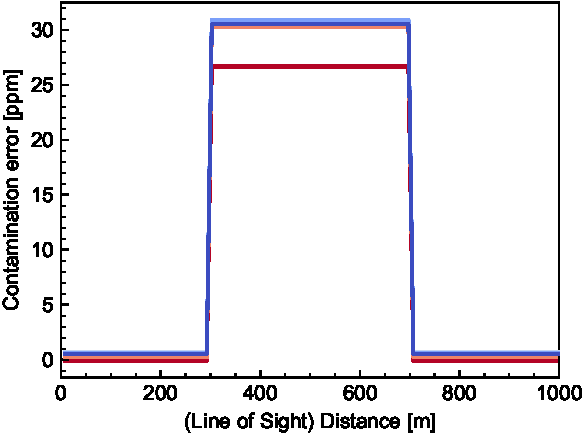
\includegraphics[scale=0.5]{fig/sim_01_6combies_cntm.pdf}
%         \caption{干渉誤差}
%         \label{fig:left}
%     \end{subfigure}
%     \hfill
%     \begin{subfigure}[b]{0.49\linewidth}
%         \centering
%         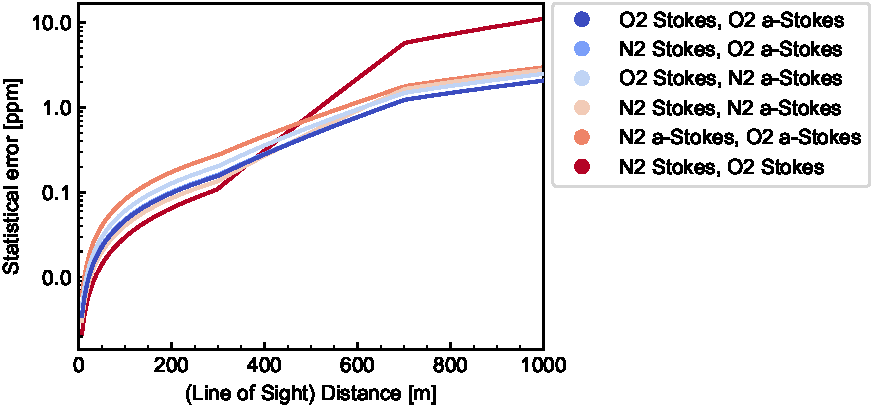
\includegraphics[scale=0.5]{fig/sim_01_6combies_stat.pdf}
%         \caption{統計誤差}
%         \label{fig:right}
%     \end{subfigure}
%     \caption{受信波長の構成による(a)干渉誤差, (b)統計誤差の比較}
%     \label{fig:two_side_by_side}
% \end{figure}

\chapter{誤差改善に向けた手法の検証}\label{chapt3}

\section{距離分解能と統計誤差の関係}
提案手法であるラマンDIALでは,
\ce{SO2}が高濃度, あるいは広範囲に分布する環境において測定を行う場合,
レーザ光およびラマン散乱光の減衰が大きくなり,
受信光子数の低下に伴って統計誤差が増大する.
そのため, \ce{SO2}濃度の変動による統計誤差の増大を考慮した
観測システムおよび信号処理手法の設計が不可欠である.

統計誤差を低減する手法として,
ライダー観測では信号加算による距離分解能の調整が一般に用いられる.
信号加算では, 計測時には距離分解能を細かく設定してライダー信号を取得し,
信号処理段階で隣接する複数距離の信号を加算することで,
その平均距離に対応する信号として扱う.
この処理により受信信号のS/Nは向上する一方,
複数距離の情報が統合されるため距離分解能は低下する.

そこで,
二酸化硫黄が豊富に存在する火山環境での観測を想定し,
信号加算の有無がラマンDIALによる測定性能に与える影響について
数値シミュレーションにより評価した.

霧島火山では,
三宅島と比較して3\sim4倍程度の二酸化硫黄濃度が報告されている.
これを参考に濃度分布を再設定した.
\cref{fig:gas_setting_SO2thick}に再設定した火山ガス濃度分布を示す.
\begin{figure}
  \centering
  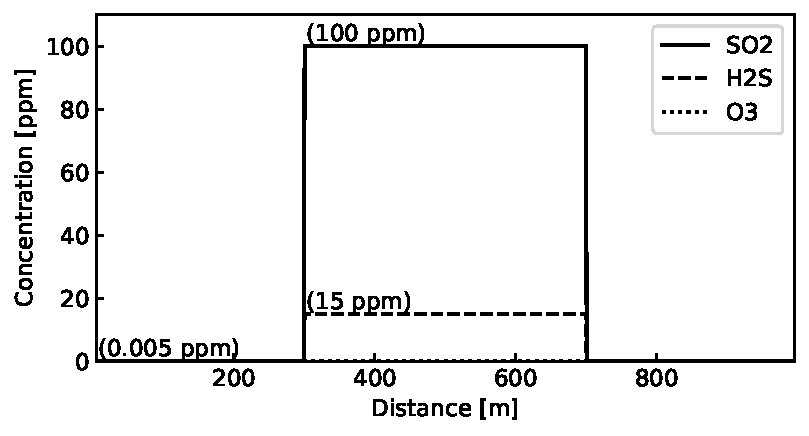
\includegraphics{fig/sim_02_1_env}
  \caption{\ce{SO2}が豊富な火山環境を想定した濃度分布設定}
  \label{fig:gas_setting_SO2thick}
\end{figure}

\noindent
\ref{chapt2}章で用いた設定から,
高濃度区間の\ce{SO2}濃度を\qty{100}{ppm}に変更している.
なお, システムパラメータは\ref{chapt2}章と同一である.

\cref{fig:fix_res}に,
距離分解能\qty{5}{m}のライダー信号から\ce{SO2}濃度を推定した場合と,
信号加算により距離分解能を\qty{25}{m}に調整した場合の
シミュレーション結果を示す.
\begin{figure}
  \centering
  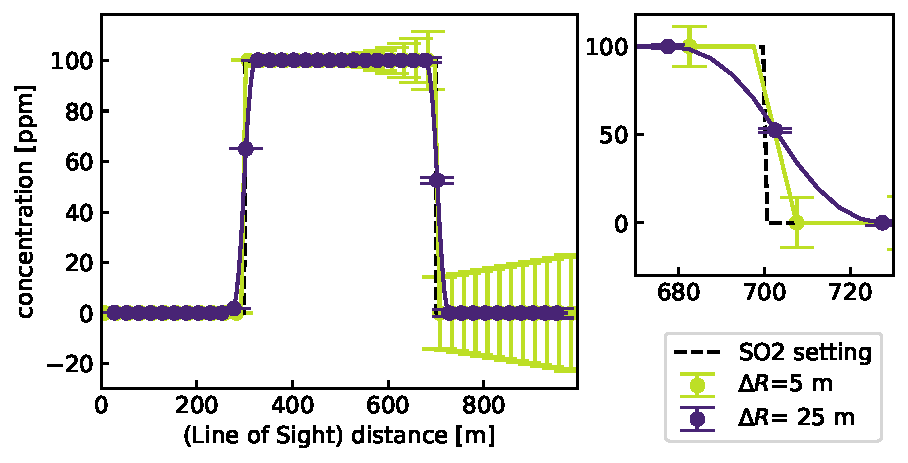
\includegraphics{fig/sim_02_1_dR-5mto25m.pdf}
  \caption{$\Delta R=5, 25 \unit{m}$による\ce{SO2}測定シミュレーション}
  \label{fig:fix_res}
\end{figure}

\noindent
横軸はライダーの視線距離, 縦軸は\ce{SO2}濃度である.
エラーバーは統計誤差を表す.
視線距離\qty{700}{m}付近の高濃度区間における測定点を比較すると,
$\Delta R=\qty{5}{m}$では\staterr が\qty{13.4}{ppm}であるのに対し,
$\Delta R=\qty{25}{m}$では\qty{1.2}{ppm}まで低減している.
一方, 実線で示す推定結果に注目すると,
$\Delta R=\qty{25}{m}$の場合には,
設定値（点線）に対する急峻な濃度変化への追従性が低下している.

\newpage
\cref{equ:stat_err}より,
統計誤差\staterr は距離分解能$\Delta R$と相反関係にあり,
信号加算によって高濃度ガスが滞留する区間における
急激な濃度変化を十分に捉えられなくなることが確認された.
信号加算前後の受信信号強度を\cref{fig:fix_power}に示す.
\begin{figure}
  \centering
  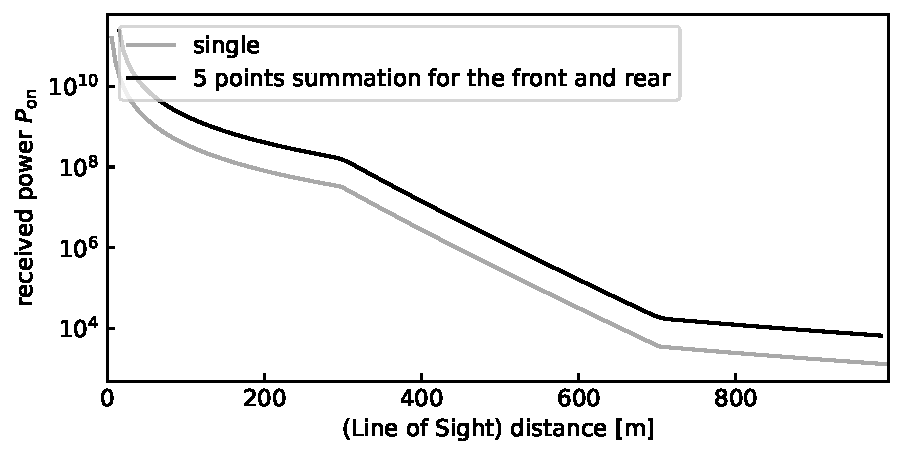
\includegraphics{fig/sim_02_1_power.pdf}
  \caption{信号加算前後の受信信号強度の変化}
  \label{fig:fix_power}
\end{figure}

\noindent
横軸は視線距離, 縦軸は受信光子数である.
単信号の信号強度を見ると,
\qty{300}{m}付近と\qty{700}{m}付近で減衰傾向が変化している.
これは, 低濃度区間では大気吸収が支配的であったのに対し,
高濃度区間では\ce{SO2}吸収が支配的となったためである.
このような信号強度の距離依存性を利用することで,
距離分解能が要求されない区間に限定して
信号加算を適用する手法が有効であると考えられる.

\newpage
\section{他ガス濃度推定による干渉誤差の補正効果}
\cref{equ:contam_err}より,
測定対象である\ce{SO2}以外の干渉ガス濃度$\subrm{n}{gas}$が高い場合,
干渉誤差\cntmerr は増大する.
\ref{chapt2}章で用いた\ce{H2S}濃度分布では,
高濃度区間の濃度を\qty{15}{ppm}としていた.
しかし, 霧島火山では\qty{100}{ppm}から\qty{2000}{ppm}程度の
\ce{H2S}濃度が報告されている.
このような環境では,
干渉誤差を無視できない可能性がある.

この場合,
干渉ガス濃度を事前に推定して\cntmerr を算出し,
\cref{equ:n_SO2}から差し引くことで,
干渉ガスの影響を低減できる.
そこで,
\ce{H2S}が豊富に存在する火山環境を想定し,
干渉誤差補正の有無が測定性能に与える影響を評価した.

\cref{fig:gas_setting_H2Sthick}に,
再設定した火山ガス濃度分布を示す.
高濃度区間の\ce{H2S}濃度を\qty{1000}{ppm}に変更している.
システムパラメータは\ref{chapt2}章と同一である.

\newpage
\begin{figure}
  \centering
  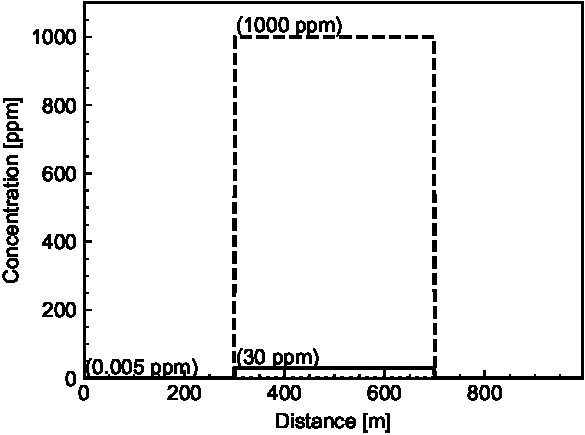
\includegraphics{fig/sim_02_2_env.pdf}
  \caption{\ce{H2S}が高濃度の火山ガス分布設定}
  \label{fig:gas_setting_H2Sthick}
\end{figure}

実観測を想定すると,
火口位置は目視等により概ね把握可能であり,
視線上で高濃度ガスが存在する区間を予測できる.
ここでは, 視線距離\qty{500}{m}に火口が存在し,
その前後\qty{100}{m}を高濃度区間と仮定した.

推定条件として, 次の5ケースを設定した.
\ce{O3}濃度は観測領域全域で\qty{0.005}{ppm}とした.
\begin{enumerate}[label=(\arabic*)]
  \item 無補正
  \item 大気および\ce{O3}を補正
  \item 大気, \ce{O3}, \qty{500}{ppm}の\ce{H2S}を補正
  \item 大気, \ce{O3}, \qty{600}{ppm}の\ce{H2S}を補正
  \item 大気, \ce{O3}, \qty{800}{ppm}の\ce{H2S}を補正
\end{enumerate}

\noindent
\cref{fig:corr_cntm}に各推定条件による
干渉補正後の\ce{SO2}濃度推定結果を示す.

\newpage
\begin{figure}
  \centering
  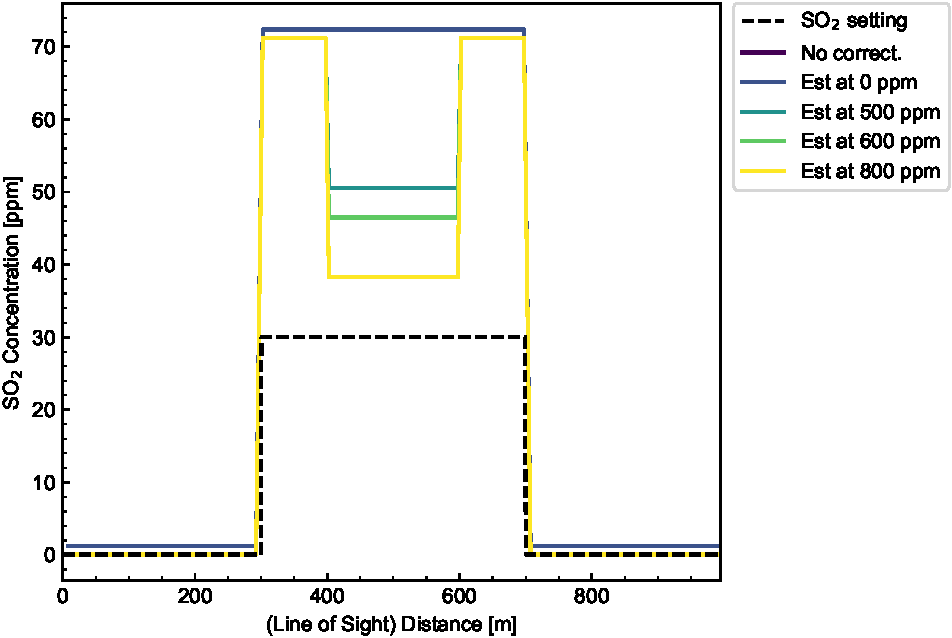
\includegraphics{fig/sim_02_2_contami_result.pdf}
  \caption{
    高濃度区間の一部について\ce{H2S}補正を行ったラマンDIALによる
    \ce{SO2}測定シミュレーション
  }
  \label{fig:corr_cntm}
\end{figure}

\noindent
補正量が大きいほど,
高濃度区間における\ce{SO2}濃度推定値は
設定値（点線）に近づく傾向を示す.
一方,
仮定した高濃度区間外である
\qty{300}{m}から\qty{400}{m},
および\qty{600}{m}から\qty{700}{m}では,
高濃度の\ce{H2S}による干渉誤差が顕著である.
干渉誤差の改善量を\cref{tab:res_cntm}に示す.
\begin{table}
  \centering
  \caption{各推定条件における\ce{SO2}濃度推定結果と濃度誤差}
  \label{tab:res_cntm}
  \begin{tabular}{ccc}
    \hline
    推定条件 & \ce{SO2}推定値 [\unit{ppm}] & 濃度誤差 [\unit{ppm}]\\
    (1) & 72.4  & 42.4\\
    (2) & 71.2  & 41.2\\
    (3) & 50.6  & 20.6\\
    (4) & 46.5  & 16.5\\
    (5) & 38.2  & 8.24\\
    \hline
  \end{tabular}
\end{table}

\noindent
大気および\ce{O3}のみを補正した場合でも,
干渉誤差は約\qty{1}{ppm}低減している.
さらに,
\ce{H2S}濃度を\qty{800}{ppm}と仮定した場合には,
干渉誤差は\qty{8.24}{ppm}まで低減した.
しかし,
設定した\ce{SO2}濃度が\qty{30}{ppm}であることを考慮すると,
十分な測定精度が得られているとは言い難い.
以上より,
干渉ガス濃度が非常に高い環境での測定は困難であることが示された.
実観測では,
干渉ガス濃度が比較的安定した火山で事前に妥当な推定値を設定する,
あるいは他手法による補助的な濃度測定と併用する必要がある.

\newpage
\section{信号加算と干渉ガス補正による効果}
本章の結論として, 
ライダー信号の処理による統計誤差の抑制について, 
$\Delta R$ を\qty{5}{m}から\qty{25}{m}として処理することで
\ce{SO2}が\qty{100}{ppm}の高濃度領域で発生する統計誤差を, 
\qty{13.4}{ppm}から\qty{1.2}{ppm}まで抑制できる. 
しかし, 濃度分布に対する追従性が悪化するため, 
信号強度の距離変化に合わせて距離分解能が要求されない区間で信号加算を行うといった柔軟な測定が有効だといえる. 
また, ラマンDIAL推定時の干渉ガス濃度の推定による補正について, 
霧島火山のような\ce{H2S}高濃度地点の測定をする際は, 
干渉誤差も濃度に従って大きくなり,
補正が困難となるため, 
事前に妥当な推定値を用意するか, 
補助的な濃度測定手法を併用する必要があることが明らかとなった. 

% \chapter[プルームモデルに従う火山ガス分布のシミュレーション]{プルームモデルに従う火山ガス分布のシミュレーション}
\label{chapt4}

本章は, これまで用いてきた区間ごとに火山ガス濃度が一定と仮定した理想モデルを発展させ,
大気中での移流および拡散を考慮したプルームモデルに基づく火山ガス分布を導入し,
より現実的な測定条件下におけるラマンDIAL観測性能について検討する.
特に, 大気の拡散条件や火口位置の違いが,
ライダー測定における距離分解能および濃度推定精度に与える影響を数値シミュレーションにより評価する.

\section{プルームモデル}

\ref{chapt3}章までは,
ある区間ごとに火山ガス濃度が一定の理想モデルで
シミュレーションを行った.
しかし, 実際の火山ガス濃度分布は大気中を拡散し,
風によって移流する.
より現実的な測定条件での検討を行うためには,
この移流拡散による濃度分布を再現する必要がある.

プルームモデルは,
流体の移流拡散方程式の解析解であり,
プラントや自動車の排煙による
大気汚染のシミュレーションに広く用いられている.
煙源を原点とした座標系における
$x, y$方向の地表面濃度は,
プルームモデルに基づいて\cref{equ:plume}で表される.

\noindent
式中の$Q$は煙源の放出強度,
$u$は風速,
$\subrm{\omega}{y}, \subrm{\omega}{z}$はそれぞれ
水平方向および鉛直方向の拡散幅,
$H_\mathrm{e}$は有効煙突高さである.
なお,
$\subrm{\omega}{y}, \subrm{\omega}{z}$の算出には,
Pasquill--Giffordが提案した大気安定度モデルを用いた\cite{pasquill,gifford}.

\section{拡散条件や火口位置による距離分解能の評価}

\cref{tab:plume_params}に,
プルームモデルに与える大気の拡散条件とパラメータを示す.
火口からの放出量は一定とし,
拡散条件の違いによる火山ガス濃度分布の変化を比較した.

\begin{table}
  \centering
  \caption{プルームモデルに与える拡散条件とパラメータ}
  \label{tab:plume_params}
  \begin{tabular}{lcc}
    \hline
          & 強拡散 & 弱拡散 \\
    \hline
    風速   & \qty{2}{m/s}  & \qty{10}{m/s} \\
    日照   & 晴れ          & 曇り          \\
    $\subrm{Q}{SO2}$ & \multicolumn{2}{c}{\qty{30e6}{kg/s}} \\
    $\subrm{Q}{H2S}$ & \multicolumn{2}{c}{\qty{7.5e6}{kg/s}} \\
    \hline
  \end{tabular}
\end{table}

2種類の拡散条件における
地表面の火山ガス濃度分布を\cref{fig:gas_map_compare}に,
ライダー視線上の火山ガス濃度分布設定を
\cref{fig:gas_setting_diffuse_compare}に示す.

\begin{figure}
  \centering
  \begin{subfigure}{0.48\linewidth}
    \centering
    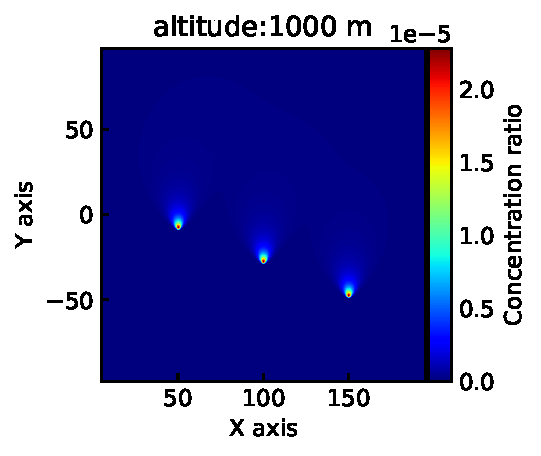
\includegraphics[width=\linewidth]{fig/sim_04_env_image1.pdf}
    \caption{強拡散大気条件}
    \label{fig:gas_map_high_diffuse}
  \end{subfigure}
  \hfill
  \begin{subfigure}{0.48\linewidth}
    \centering
    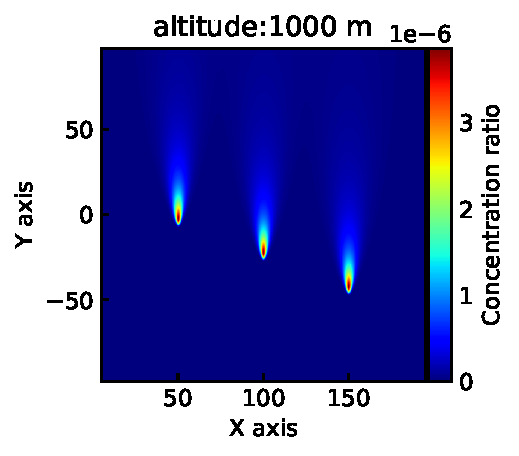
\includegraphics[width=\linewidth]{fig/sim_04_env_image2.pdf}
    \caption{弱拡散大気条件}
    \label{fig:gas_map_low_diffuse}
  \end{subfigure}
  \caption{大気拡散条件の違いによる地表面火山ガス分布}
  \label{fig:gas_map_compare}
\end{figure}

\begin{figure}
  \centering
  \begin{subfigure}{0.48\linewidth}
    \centering
    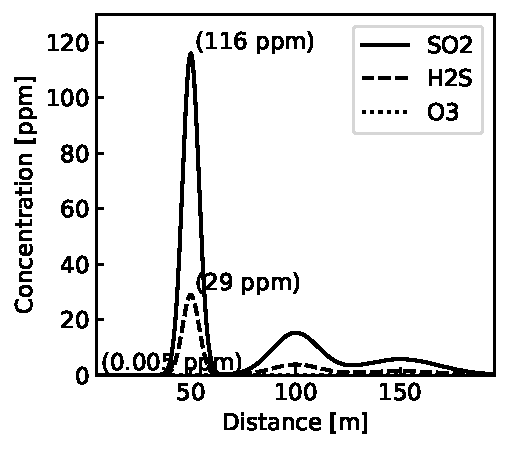
\includegraphics[width=\linewidth]{fig/sim_04_env1.pdf}
    \caption{強拡散大気条件}
    \label{fig:gas_setting_high_diffuse}
  \end{subfigure}
  \hfill
  \begin{subfigure}{0.48\linewidth}
    \centering
    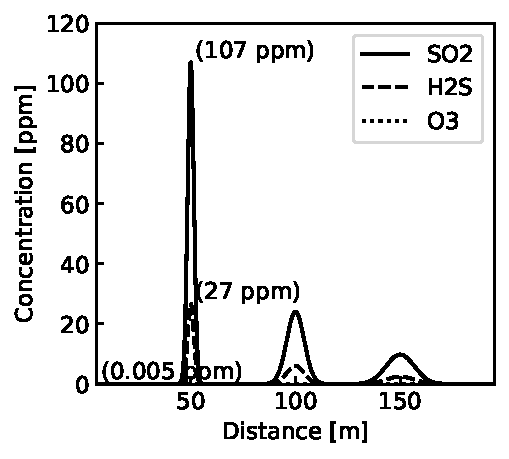
\includegraphics[width=\linewidth]{fig/sim_04_env2.pdf}
    \caption{弱拡散大気条件}
    \label{fig:gas_setting_low_diffuse}
  \end{subfigure}
  \caption{大気拡散条件の違いによるライダー視線上の濃度分布設定}
  \label{fig:gas_setting_diffuse_compare}
\end{figure}

\begin{figure}
  \centering
    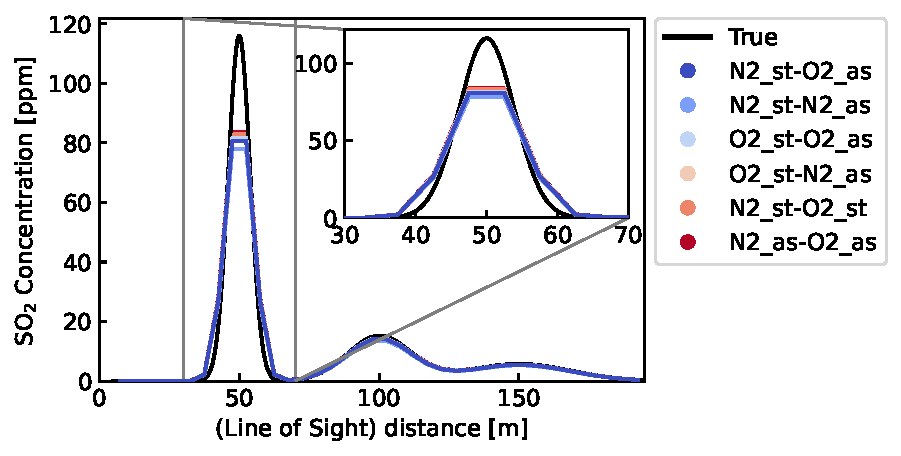
\includegraphics{fig/sim_04_plume_meas1.pdf}
    \caption{強拡散大気条件場における\ce{SO2}測定シミュレーション}
    \label{fig:plume_meas_high_diffuse}  
\end{figure}

\begin{figure}
  \centering
    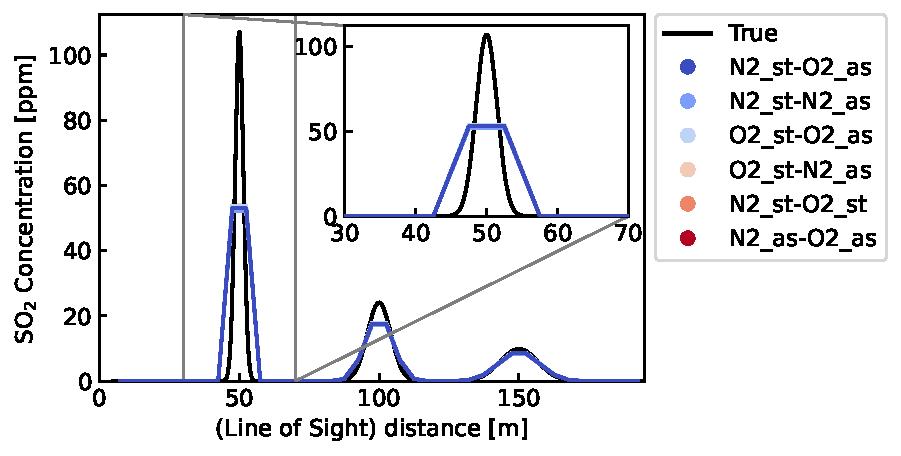
\includegraphics{fig/sim_04_plume_meas2.pdf}
    \caption{弱拡散大気条件場における\ce{SO2}測定シミュレーション}
    \label{fig:plume_meas_low_diffuse}  
\end{figure}

% \chapter[結論]{結論}\label{chapt5}

% % -=-=-=-=-=-=-=-=-=-=-=-=-=-=-=-=-=-=-=-=-=-=-=-=-=-=-=-=-=-=-=-=-=-=-=-=-=-=-
%  thanks.tex - 謝辞ページ
% -=-=-=-=-=-=-=-=-=-=-=-=-=-=-=-=-=-=-=-=-=-=-=-=-=-=-=-=-=-=-=-=-=-=-=-=-=-=-
% ★謝辞
{ \setlength{\parskip}{0.7em}

\chapter*{謝辞}

本研究の遂行にあたり,
指導教員として終始多大なご指導とご助言を賜りました
柴田泰邦教授に深く感謝申し上げます.
研究の方向性に関する助言から, 
論文執筆に至るまで丁寧にご指導いただき,
本研究をまとめ上げる上で多くの学びを得ることができました.
ここに記して, 
心より深謝致します.

同学域の田川憲男教授,
並びに坂本高秀准教授には,
本論文の作成にあたり, 
副査として的確なご助言を賜りました.
ここに深く感謝の意を表します.

同研究室の同級生, 後輩の皆さんには,
合同ゼミや日々の議論を通して, 
研究を進める上で多くの示唆をいただきました.
ここに記して感謝申し上げます.

最後に, 
本研究に関わっていただいたすべての皆様に深謝の意を表し,
本論文の謝辞とさせていただきます.

}


\printbibliography[title=参考文献]
% % -=-=-=-=-=-=-=-=-=-=-=-=-=-=-=-=-=-=-=-=-=-=-=-=-=-=-=-=-=-=-=-=-=-=-=-=-=-=-
%
%  卒業論文用テンプレート
%  appendix.tex - 「付録」ページ
%
%  自分の卒論にあわせてこのファイルの★印部分を必要に応じて変更しましょう．
%  ※付録を付けない場合はこのファイルをincludeする必要はありません
%
% -=-=-=-=-=-=-=-=-=-=-=-=-=-=-=-=-=-=-=-=-=-=-=-=-=-=-=-=-=-=-=-=-=-=-=-=-=-=-

\appendix

% -=-=-=-=-=-=-=-=-=-=-=-=-=-=-=-=-=-=-=-=-=-=-=-=-=-=-=-=-=-=-=-=-=-=-=-=-=-=-
\chapter{　　　} \label{Rnet_information}


\end{document}
